

\chapter{Nbody application}


After the previous analytical study, we present here the characteristics of  numerically obtained Hubble-Lema\^itre fragmented models. The integration was performed with NBODY6, which treats the gravitational forces of stars with no softening of the potential. An example of the evolution of the system is shown on Fig~\ref{Fig:2_fragmentation}. 


\section{Approaching the N-body simulations}



\begin{figure}[h]
\begin{center}
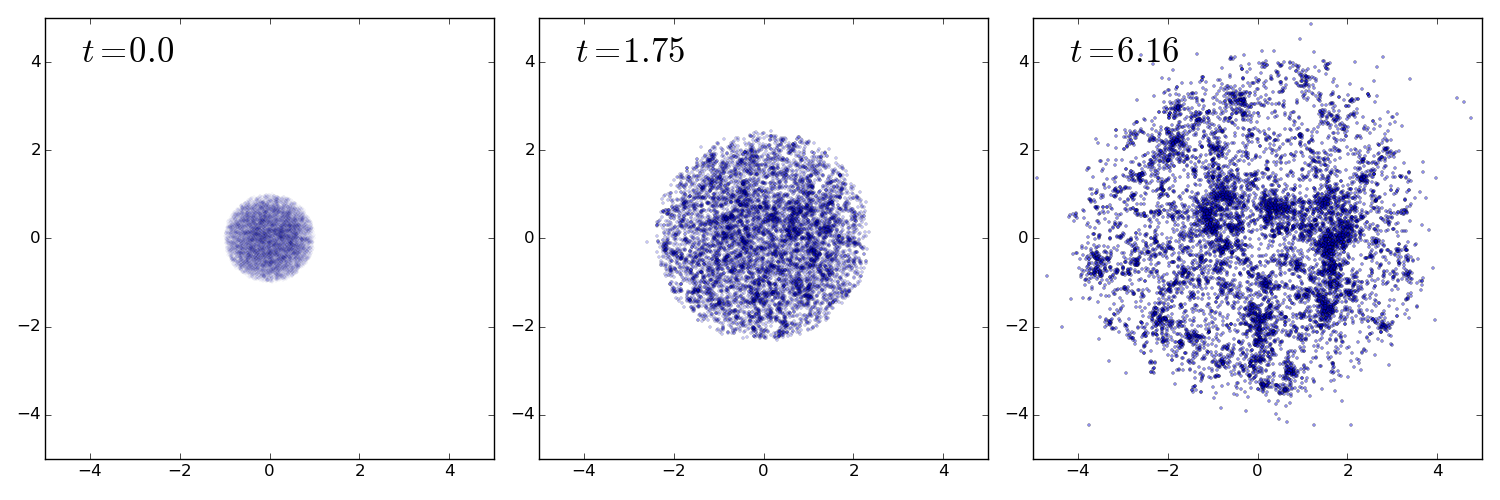
\includegraphics[width=\textwidth]{Figures/2_fragmentation}
\caption{Progressive fragmentation through the Hubble expansion. The left panel shows the initial uniform sphere; the middle panel, an intermediate step, slightly fragmented with a slowed down expansion; the right panel is the final stage, when the expansion has stopped and the fragmentation is fully developed. N=10000 particles were used in this N-body model, with $\Hub_0 = 1.0$. Time and coordinates are in H\'enon units.}
\label{Fig:2_fragmentation}
\end{center}
\end{figure}

\subsection{Presentation of the runs}

We draw $N$ stars from an Salpeter distribution function which we truncate by default to $100 M_\odot$~; in some calculations we will  use a lower bound of $20 M_\odot$, and in others we use identical masses. The code preserves the total energy and angular momentum to better than one part in $10^4$ for integration over $\sim 100 $ time units.  

\subsection{Clump finding algorithm}

As seen on Fig~\ref{Fig:2_fragmentation}, once expansion stops, the distribution is roughly spherical and visibly clumpy. By clump we mean here a local overdensity of stars. To characterize the model, it is necessary to find and isolate clumps, using an efficient clump-identification algorithm (or, {\it halo-finding} in cosmology).  Several methods are commonly used such as the HOP algorithm \citep{Eisenstein1998,Skory2010} which relies on attributing local densities to each particle and separating the clumps through density thresholds. The HOP algorithm is very robust on large cosmological data sets. However, our calculations have comparatively coarse statistics and noisy density fields. This issue, coupled with the  large number of free parameters of the HOP algorithm, makes the method less appealing. 

Instead we follow \cite{Maschberger2010} who adapted the minimum spanning tree (MST~; see e.g. ~\citealt{Allison2009b,Olczak2011}) technique to the detection of clumps. A spanning tree is a set of edges connecting a group of  particles without closed loops~; the MST seeks to minimise the total length of the edges. One may then construct the MST for the whole system, and then delete all edges larger than a chosen cutting length, $d_{cut}$. The sub-sets that are still connected  are labeled as clumps. This process is illustrated in Fig \ref{Fig:2_MST}. In practice a minimum sub-set size $N_d$  is also chosen so as to avoid many small-N subgroups~: experience led us to choose  $N_d = 12$ for the minimum number of stars per clump. 

\begin{figure}[h]
\begin{center}
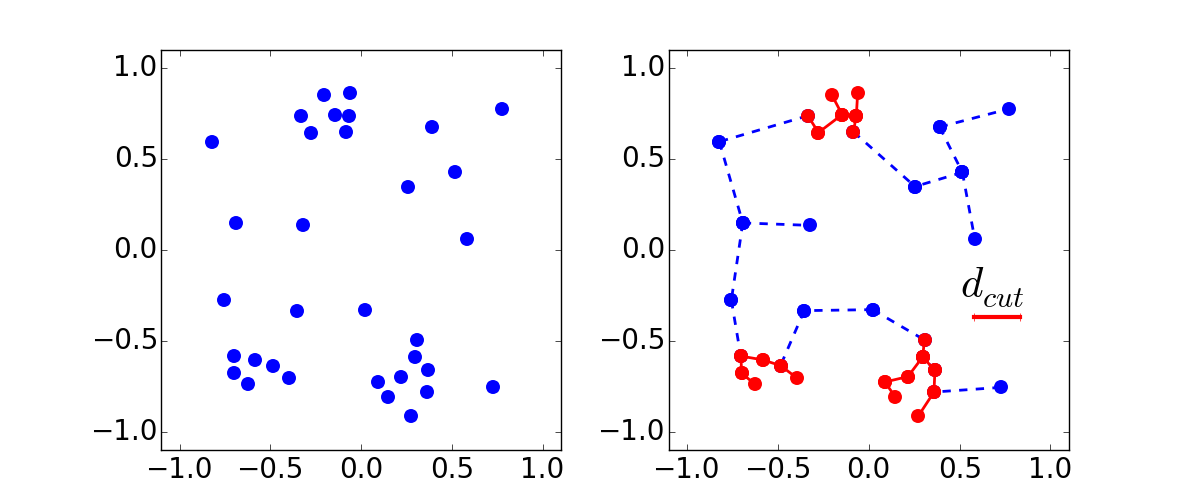
\includegraphics[width=0.8\columnwidth]{Figures/2_MST.png}
\end{center}
\caption{Illustration of a Minimum Spanning Tree and its use to isolate subgroups, using a cutting length $d_{cut}$.}
\label{Fig:2_MST}
\end{figure}


With $N_d$ fixed, the length $d_{cut}$ is then the only free parameter left. There is some freedom 
in choosing an appropriate value. \cite{Maschberger2010} fixed the value of  $d_{cut}$ by visual inspection of clumps.  We instead  identified  clumps in a fragmented system for a range of values for $d_{cut}$ and settled for the value  which optimised the number of identifications. This is shown on Fig.~\ref{Fig:2_Ndcut} for an N = 80k fully-fragmented Hubble model. For small values of $d_{cut}$, the number of detected clumps at first  increases rapidly. The rise is due  to the length $d_{cut}$ initially being small compared with the typical volume spawned by $N_d$ or more  nearest-neighbours. Beyond a certain value, a transition to another regime occurs, whereby the algorithm starts to connect previously separated clumps, counting them as one. The number of clumps thereafter begins to decrease. The value $d_{cut} \approx 0.023$ H.u optimises the outcome of the clump-search. This is a generic feature of the MST algorithm and we have adopted the same strategy throughout, adapting the value of $d_{cut}$ to the number $N$ of stars used. 


 \begin{figure}
\center
    \centering
    \begin{subfigure}[b]{0.49\textwidth}
    	\centering
    	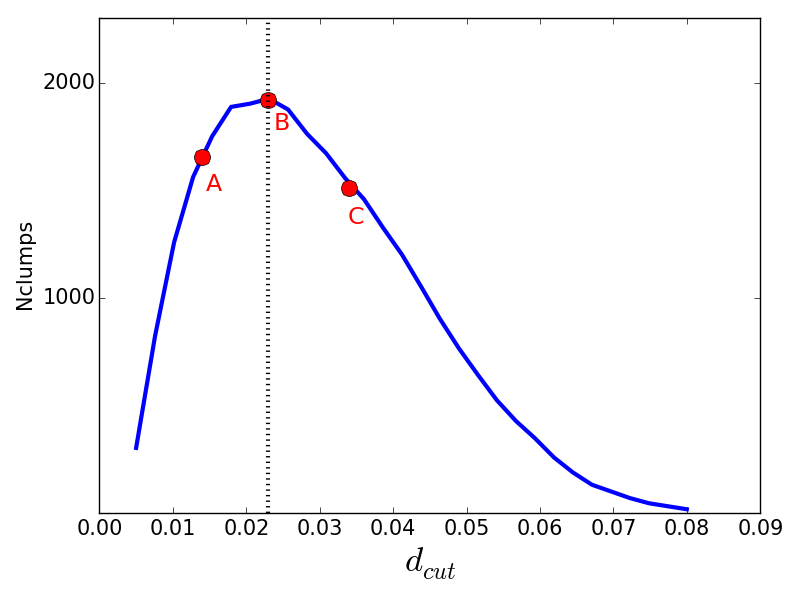
\includegraphics[width=\textwidth]{Figures/2_Ndcut.png}
        \caption{Number of clumps vs $d_{cut}$}
        \label{Fig:2_Ndcut}
    \end{subfigure}
    \begin{subfigure}[b]{0.49\textwidth}
    	\centering
    	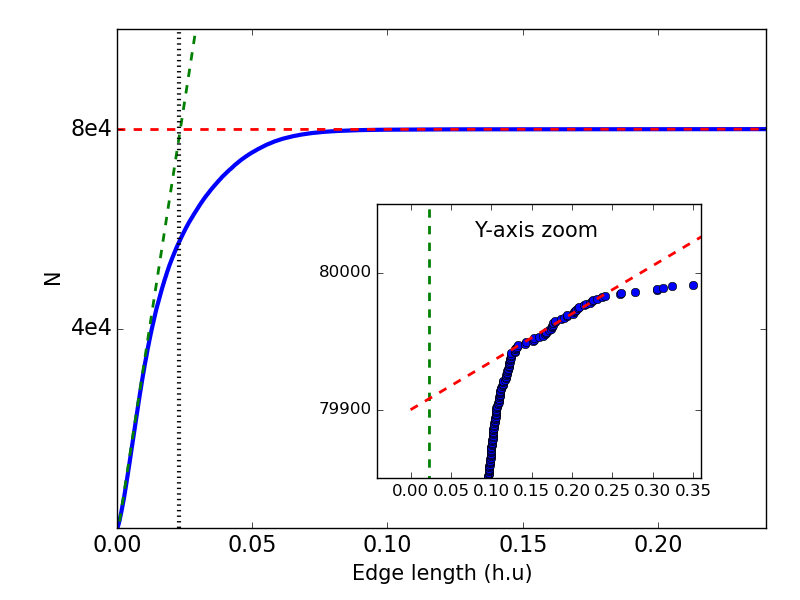
\includegraphics[width=\textwidth]{Figures/2_dcutdistribution.png}
        \caption{Cumulative distribution of MST edges}
        \label{Fig:2_dcutcumulated}
    \end{subfigure}
\caption{Two different methods to identify the critical $d_{cut}$ for clump detection. Both methods give the same value. For this 80k model, the value is 0.023 in H\'enon units. The red linear fit on (b) was made on the linear portion with sufficient data points, discarding the very few further points departing from the tendency.}
\label{Fig:0_dcutchoice}
\end{figure}


 

 


\begin{figure}[h]
\begin{center}
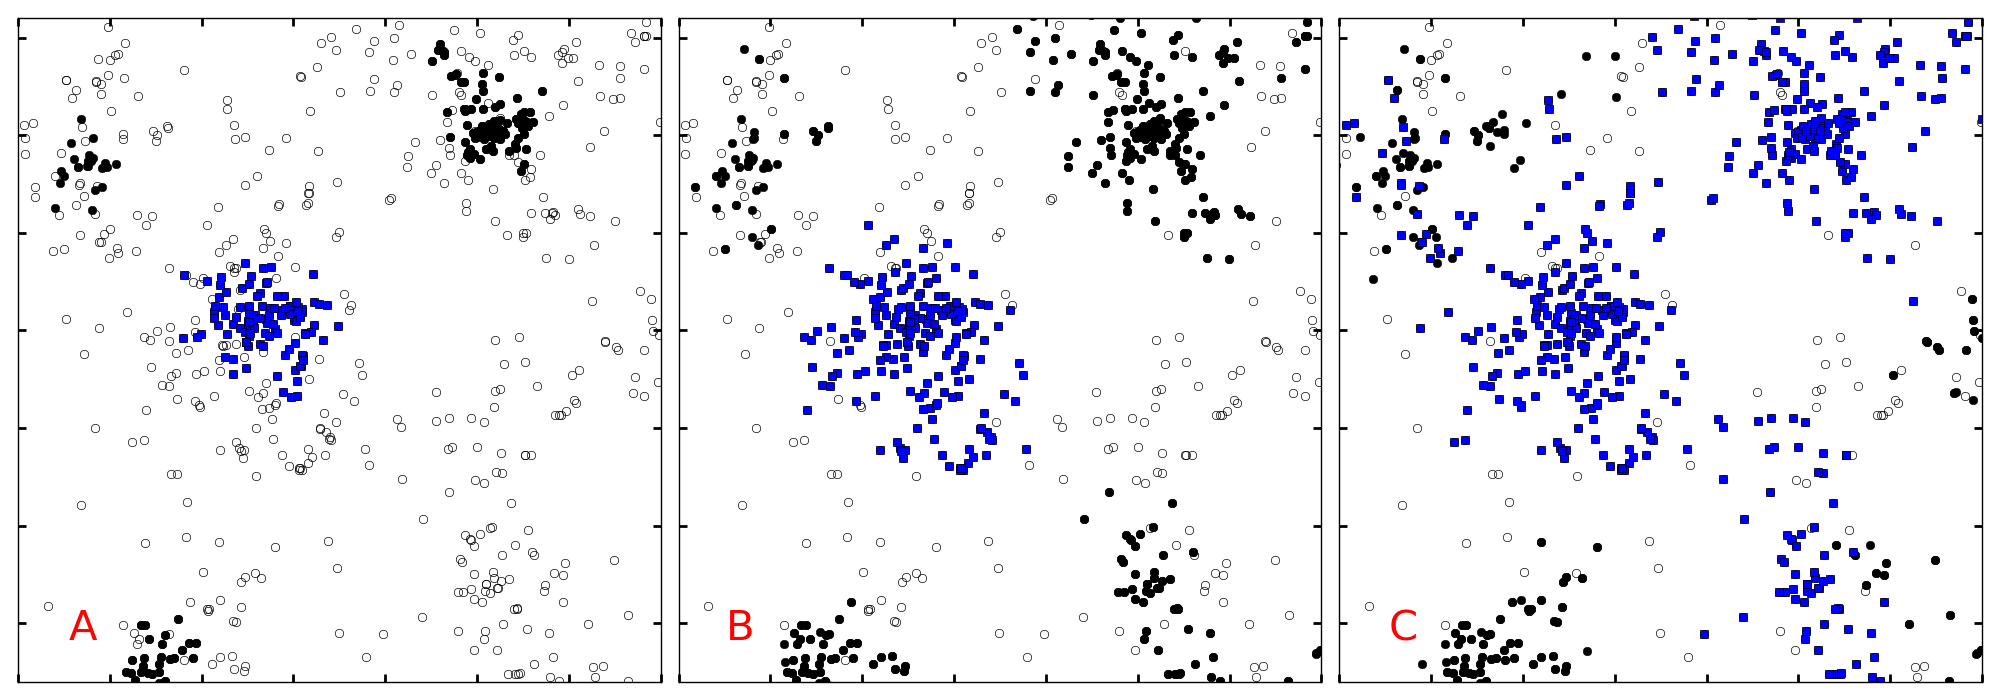
\includegraphics[width=\columnwidth]{Figures/2_clumpsABC.png}
\end{center}
\caption{Example of detected clumps for three cutting length, 0.014 (top panel), 0.024 (middle panel), 0.034 (bottom panel), which were labeled A,B,C  in Fig.~\ref{Fig:2_Ndcut}. A cube within a 80k particles fragmented model was extracted and projected.  Empty circles are stars which do not belong to any clump, black circles are clump members, and blue squares are stars that are identified as a single large  clump. Tick marks are spaced by 0.05 length units for a box size of 0.35 units.}
\label{Fig:2_clumpsABC}
\end{figure} 




Another method to find the critical cutting length was used by \cite{Gutermuth2009,Kirk2011}. In these works, the authors build the MST, then trace the cumulative distribution function of all edges in the tree. In a clumpy configuration, there are at least two regimes: the "intra-clump" regime, with the majority of small edges, and the "inter-clump" regime with longer, scarcer edges. The intersection of the linear fits to these regimes provide a good cutting length for clump detection. This procedure was applied to our system and gave the same result than the clump count, as shown on Fig~\ref{Fig:2_dcutcumulated}.

 
   On Fig.~\ref{Fig:2_clumpsABC}, a sub-set of our 80k model is shown; we have identified stars that belong to clumps with filled symbols. The three panels on that figure are each for a different value of $d_{cut}$, increasing from top to bottom. For the smallest value $d_{cut}$=0.013 H.u, clumps look somewhat truncated as we are still in the under-sampling regime and only their cores registered as clumps. The second, optimal, value $d_{cut}$=0.023 H.u produces visually well-isolated clumps. Finally, the third and  largest value is so that clumps begin to merge together~: this is shown by the unique clump identified in the bottom panel (filled blue squares).
   
   
   
   
\section{Clump mass function}

The numerical realizations of the \HubLem model allows to assess the influence of important parameters on the fragmentation, such as \tHub, N and the stellar mass function. 


\subsection{Influence of H and N}

We wish to evaluate the influence of $\Hub_0$ and N on the fragmentation and clump growth. $\Hub_0$ tunes the strength of the expansion, which tunes the duration of the fragmentation. A stronger initial expansion allows for more time for clumps to grow, so we expect more massive clumps with increasing $\Hub_0$. On the other hand, a higher N smooths the spatial distribution, reducing Poisson noise in the  distribution. However, a high membership only samples more stars from the same stellar mass function, and the density fluctuations should not change in nature, just scale down with the average distance between stars.  We do not expect N to significantly affect the fragmentation in physical units. 

To verify these, a set of simulation was performed to explore the mass function of clumps in the $\Hub_0$-N parameter space. The models have 5 different memberships that go as powers of 2 in thousands, with an increasing sampling to obtain acceptable statistics:
\begin{center}
\begin{tabular}{l|rrrrr}
\centering
N   & 1000 & 2000 & 4000 & 8000 & 16000\\ 
\hline
Sampling & 12 & 8 & 5 & 5 & 5\\
\end{tabular}
\end{center}
Each one of these models were performed with 5 different $\Hub_0$:
\begin{center}
\begin{tabular}{l|rrrrr}
$\Hub_0$ & 0.8 & 0.9 & 1.0 & 1.1 & 1.2
\end{tabular}
\end{center}
for a total of 175 different models ran up to the end of the expansion. The stars are taken from a Salpeter mass function with a $[0.3, 100] M_\odot$ mass range. 

\subsubsection*{Apex time}
In section \ref{Sec:1_apextime}, we derived an analytical prediction for the apex time of our expanding models. To compare our numerical realizations to this prediction,  we follow for each model the evolution of the half-mass radius over time, then take the apex time as the maximum radius time, when the cluster stops expanding and starts collapsing. 


\begin{figure}
\begin{center}
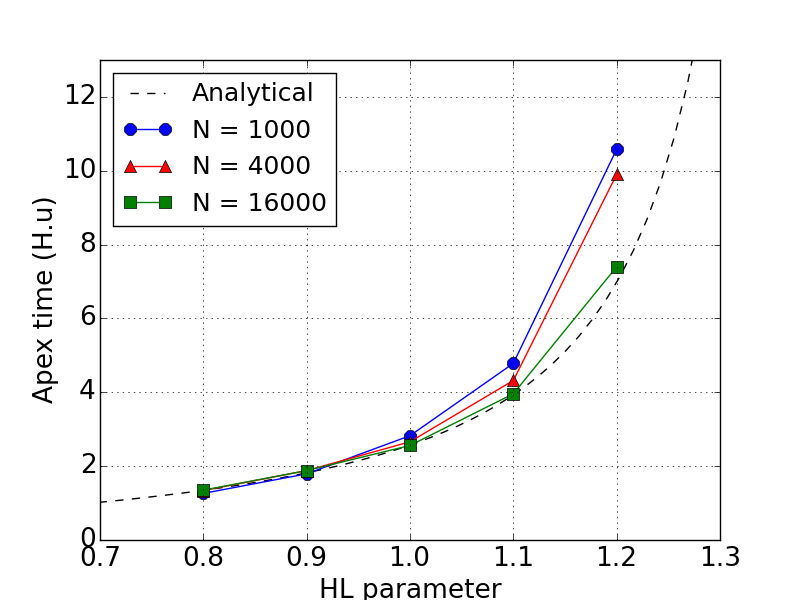
\includegraphics[width=0.6\textwidth]{Figures/2_apextime_NH.png}
\end{center}
\caption{Analytical and simulated apex times as a function of \tHub.}
\label{Fig:2_apextime_NH}
\end{figure} 

We show on Fig~\ref{Fig:2_apextime_NH} the expected analytical curve as a dashed line, then the numerically obtained apex times from our different \tHub and memberships, averaged over all similar runs. The 16k runs follow the analytical expectation within 5\%, while lower membership models take more time than expected to stop expanding at high \tHub, overshooting by as much as 30\% for \tHub =1.2. Visual inspection of the runs showed that low memberships were more susceptible to have a clump "take over" during the expansion. As we will show in the present section, low-N clusters contains more massive clumps in relative mass than high-N models. When a massive enough clump form during the expansion, it offsets the matter distribution and skews the half-mass radius (computed from the barycenter of the full system) to higher values, offsetting its fall from the collapse. To reduce unwanted "sur-fragmentation" effect, we use analytical apex times to select our fragmented configurations.  


\begin{figure}
\begin{center}
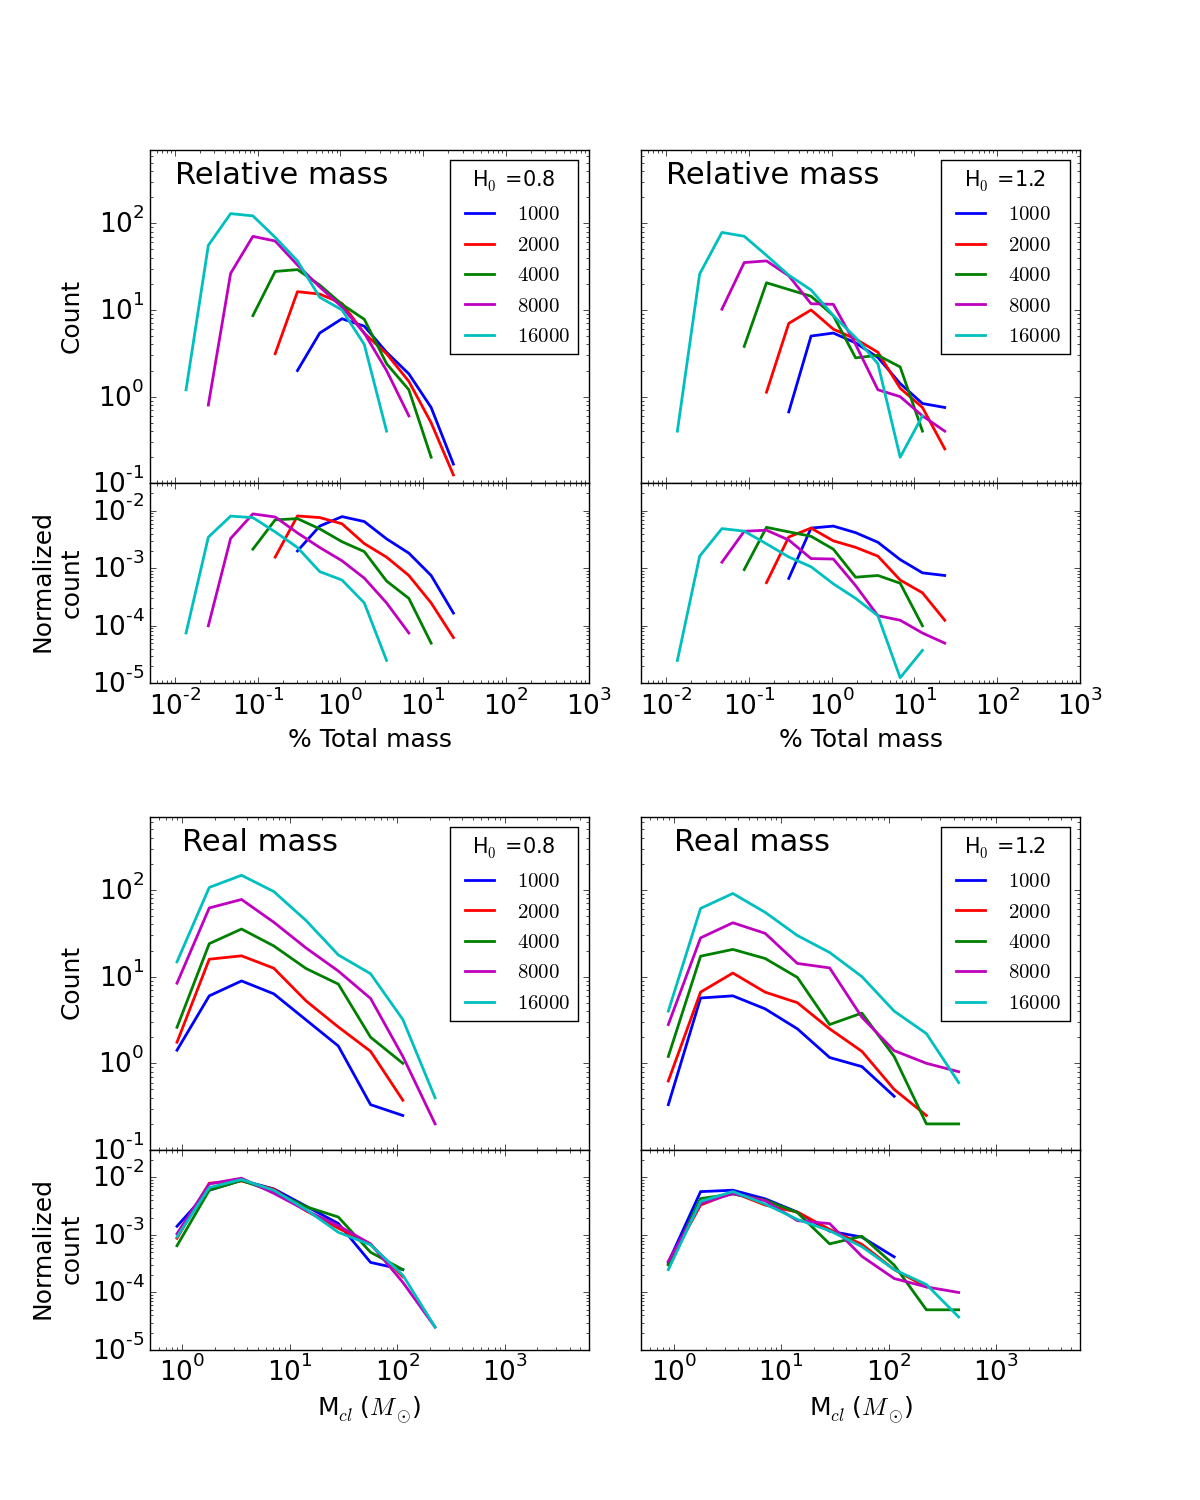
\includegraphics[width=\columnwidth]{Figures/2_ClumpMF_N.png}
\end{center}
\caption{Clump mass function for several memberships and two $\Hub_0$. Masses in the top panels are in H\'enon units, the x-axis was scaled with a factor 100 to get a percentage of the total mass of the system. Bottom panel masses are in physical units. In each panel, top sub-panel shows actual clump count in each bin (averaged over sampling), while bottom sub-panel normalize the count by the model membership. }
\label{Fig:2_ClumpMF_N}
\end{figure} 

\begin{figure}
\begin{center}
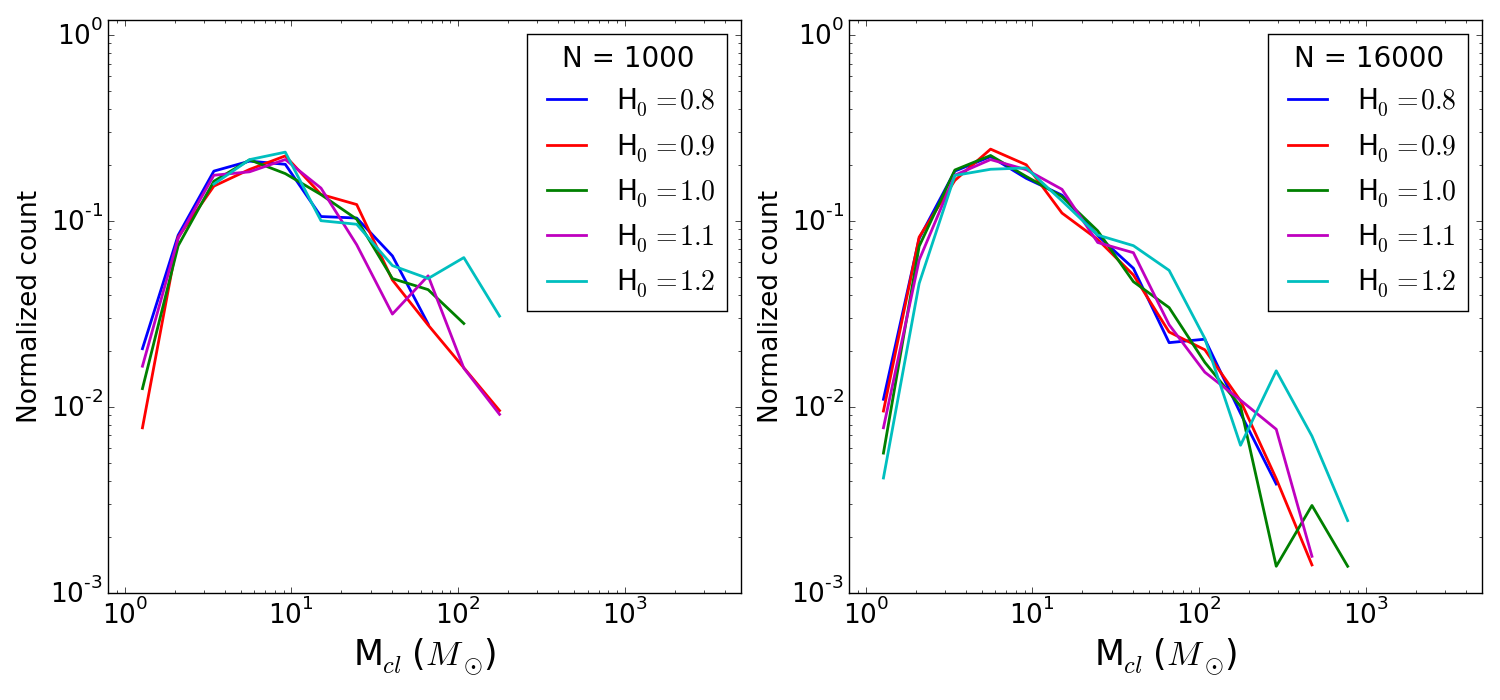
\includegraphics[width=0.95\columnwidth]{Figures/2_ClumpMF_H.png}
\end{center}
\caption{Clump mass function (real mass) for several $\Hub_0$  and two memberships.}
\label{Fig:2_ClumpMF_H}
\end{figure} 


\subsubsection*{Clump mass function}
 The clump-finding algorithm was ran on the fragmented models to obtain the clump mass function. The results are summarised as histograms on figures \ref{Fig:2_ClumpMF_N} and \ref{Fig:2_ClumpMF_H}.We have used bins of constant logarithmic intervals. We average the results over each model's sampling, hence the histogram can go down to fractional values.
 
 Looking at the top panels of Fig~\ref{Fig:2_ClumpMF_N}, we see the mass function of clumps in \textit{relative} mass, the percentage of total mass they contain.  Clumps in small-N systems tends to contain a much larger portion of the total system mass than in large-N systems, which is even clearer in the normalized count sub-panels. In fact, for \tHub = 0.8, the peak of the mass function for N=1k happens at 1.1\% of total mass, while for N=16k, it happens at 0.07\%. These values ratio gives $\sim$ 16, the membership ratio: the clumps relative masses are inversely proportional to the model's membership.
 
This can be interpreted as a underlying common clump distribution in physical mass, regardless of the total membership of the model. This is confirmed by looking at the bottom panels of Fig~\ref{Fig:2_ClumpMF_N}, in which clump distributions are plotted in physical mass, once the masses of stars have been rescaled from H\'enon units to match the original stellar mass function. Looking at the normalized count subpanels, it is clear that 1k and 16k models have the same clump distribution, when raw count subpanels show clumps are expectedly more numerous in high-N models. The difference between \tHub = 0.8 and 1.2 is not clear from the graph, but it seems a higher \tHub pushes the upper limit of the distribution to slightly higher masses.

To illustrate this last trend, we turn to Fig~\ref{Fig:2_ClumpMF_H} where clump MF are shown for various \tHub and a common membership. For  both N=1k and N=16k, the distribution preserves its shape for various \tHub, and gets prolonged at higher clump masses for N=16k, as more mass is available to build clumps.

 Thought the distribution does not undergo any dramatic change, a weak trend with \tHub is seen in both panels: as the strength of expansion increases, the distribution slightly decreases at low clump masses and slightly increases at higher clump masses, the pivot masse being $\sim$ 30 $\Mo$. We look at the 16k model and follow the cumulated mass inside all clumps, as well as the percentage of this mass in clumps below and above 30 $\Mo$, for different \tHub:

\begin{center}
\begin{tabular}{l|rrrrr}
\centering
\tHub   & 0.8 & 0.9 & 1.0 & 1.1 & 1.2\\ 
\hline
$M_{tot}$ & 3502 & 3478 & 3582 & 3683 & 3561\\
$ < 30 \Mo$(\%) & 66 & 65 & 55 & 49 & 44\\
$ > 30 \Mo$(\%) & 34 & 35 & 45 & 51 & 56\\
\end{tabular}
\end{center}

From this data, we get two facts about our fragmented models: the mass contained in clumps does not depend on \tHub ($<$2\% dispersion) and there is a transfer of mass from small clumps to more massive ones as the expansion lasts longer.

To summarise: the general shape of the clump mass function is common to all membership and \tHub. In physical mass, the same clumps form in 1k and 16k models, almost regardless of the duration of the expansion. We note a mass transfer from small to high mass clumps when \tHub increases, that is consistent with a merging process: small clumps assemble or get accreted by large clumps. When the initial expansion is strong, the merging lasts longer and more mass in transferred. This is confirmed by visual inspection of the models, as we see clumps merging during the expansion.




\subsection{Influence of stellar mass function}
\label{Sub:2_ClumpMF_MF}





\begin{table}
\begin{center}
\caption{Summary of fragmentation models and their characteristics. These simulations started from an uniform sphere and were stopped when the expansion halted, at t=3 H.u . The third column shows the number of independent computations for each model.}
\label{Tab:2_fragmentationmodels}
\begin{tabularx}{0.7\textwidth}{XXXX}
\hline
Name & N & Sampling & Mass range  \\
\hline
Rmh20 & 15000 & 30 & [0.35- 20 ]\\
Rmh100 & 15000 & 30 & [0.3 - 100]\\
Rmh1 & 15000 & 30 & 1.0 \\
\hline
\end{tabularx}
\end{center}
\end{table}



Neither \tHub or N seem to heavily influence the shape of the clump mass function. We now turn to another parameter: the stellar mass function. We know the clumps are seeded by density fluctuations in the initial uniform sphere. These fluctuations are governed by pure Poisson noise in the case of identical stellar masses, but are modified and enhanced once stars follow a mass function themselves: a high-mass star surrounded by lighter ones will by itself introduce a localized strong density fluctuation. We expect a relation between the clump mass funtion and  the {\it stellar} mass function in the generated initial conditions.

We wish to quantify this relation. To this end, we ran a set of simulations where all the stars have the same mass, and two sets for which a Salpeter mass function with $\alpha = 2.35$  was truncated at different upper- and lower-bounds. A total of 15000 stars in a Hubble configuration were used, all let go  with the same initial expansion rate  $\Hub_o = 1$. For the multi-mass models, the mass range  was chosen as $[0.3, 100]\, M_\odot$ and $[0.35, 20]\, M_\odot$ so that the mean stellar mass $= 1M_\odot$ as for the single-mass models. Thirty different runs were performed in each case and the outcome averaged for better statistics. These are refered to as Rmh1, Rmh100 and Rmh20 in Table \ref{Tab:2_fragmentationmodels}.

On Fig.~\ref{Fig:2_ClumpMF_MF}, we display the  number of clumps as function of clump mass for the truncated Salpeter  models as a red solid line, while the single stellar mass models are shown in green dash. A grey shade indicates one standard deviation where statistics allow ({\it i.e.}, large numbers), and, as in previous section, we have used bins of constant logarithmic mass intervals.  Fig.~\ref{Fig:2_ClumpMF_MF_1} shows Rmh20 models, and \ref{Fig:2_ClumpMF_MF_2} shows Rmh100 models. 
With clump membership restricted to $N \geq 12$, the identical-mass model  stays relatively close to a power law (straight dotted line on the figure) of index $\approx -4$ for the higher mass clumps. A spread in stellar masses leads to much more massive clumps (we counted $\simeq80$ clumps of $12 M_\odot$ for the equal-mass case~; and $\approx 32$ with a mass $ \le 12 M_\odot$ for the other ones) . This transforms the clump mass function, from a near-power-law, to a bell-shaped distribution.  





 \begin{figure}
\center
    \centering
    \begin{subfigure}[b]{0.49\textwidth}
    	\centering
    	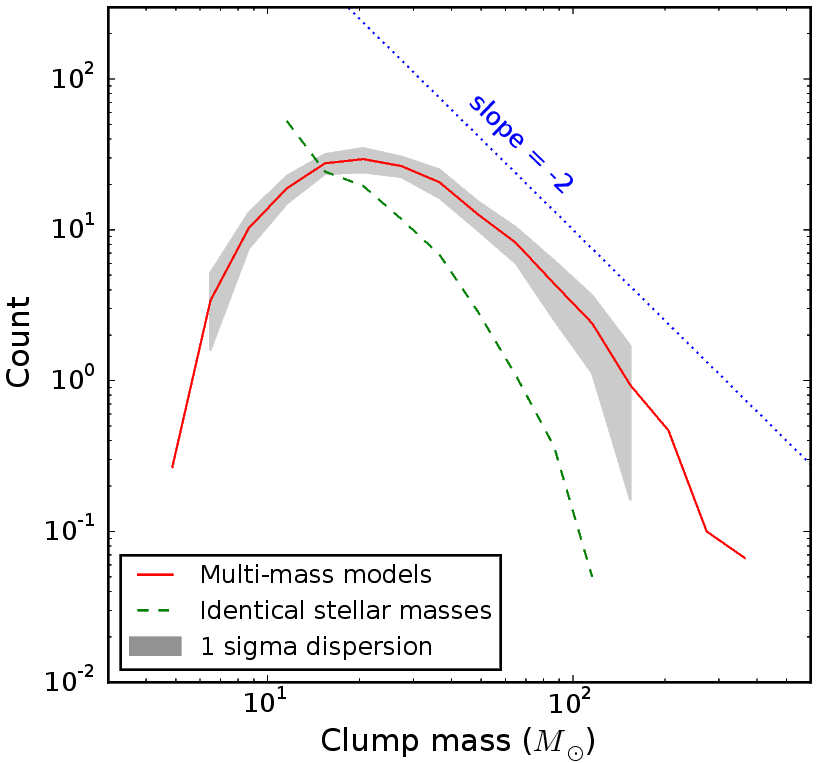
\includegraphics[width=\textwidth]{Figures/2_ClumpMF_MF_1}
        \caption{Stellar mass range $[0.35, 20]\, M_\odot$ }
        \label{Fig:2_ClumpMF_MF_1}
    \end{subfigure}
    \begin{subfigure}[b]{0.49\textwidth}
    	\centering
    	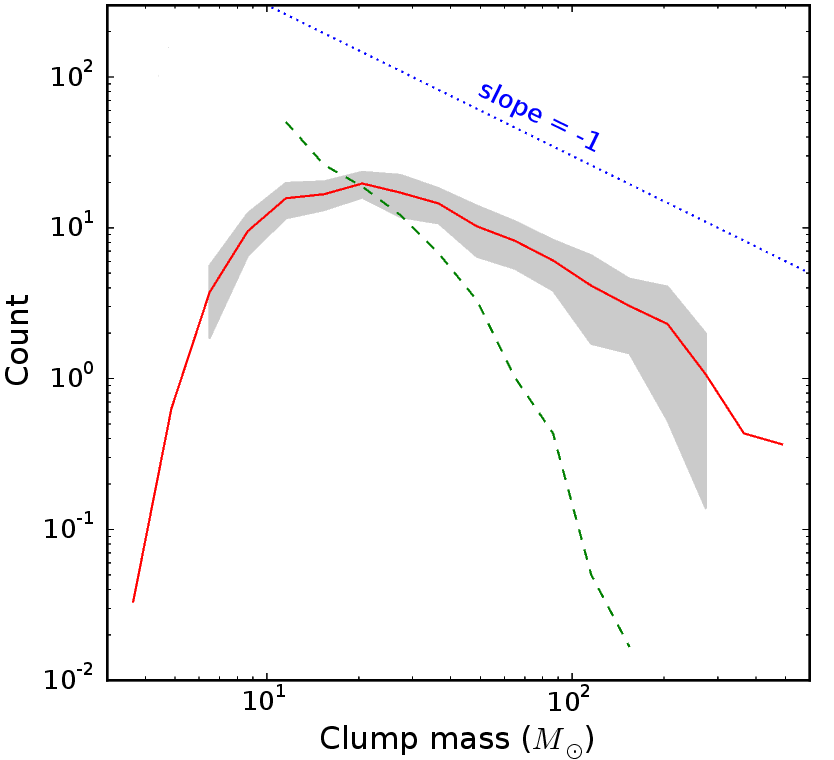
\includegraphics[width=\textwidth]{Figures/2_ClumpMF_MF_2}
        \caption{Stellar mass range $[0.3, 100]\, M_\odot$}
        \label{Fig:2_ClumpMF_MF_2}
    \end{subfigure}
\caption{Mass function of the clumps identified with the MST algorithm. The calculations all had $N = 15 000$ stars, and we have averaged over 30 realisations for each configuration.  The results for three stellar mass functions  are displayed~: a model with equal-mass stars (green dashed line)~; a Salpeter distribution function truncated at $20 M_\odot$ (solid red line, left)~; a Salpeter distribution function truncated at $100 M_\odot$(solid red line, right). (a) The clumps  mass function for equal-mass models  shows a trend with mass roughly in agreement with an $M^{-4}$ power-law. By comparison,  the results for an  Salpeter stellar distribution function  truncated at $20 M_\odot$ has a bell-shaped profile, with a peak around $M = 20.5 M_{\odot}$~; only the tail-end shows marginal agreement with an $\propto M^{-1.7}$ power-law (dotted line on the figure)~; (b) another Salpeter distribution function but with  the upper-mass truncation  set at $100 M_\odot$. The tail at large clump mass is now much flatter, with a slope $\approx M^{-1}$, (dotted line on the figure as well). The bins used  had constant logarithmic mass intervals.}
\label{Fig:2_ClumpMF_MF}
\end{figure}



When very massive stars are included in the calculations, yet more massive clumps are formed (Fig.~\ref{Fig:2_ClumpMF_MF_2}). The formation of large sub-structures depletes the number of clumps around the peak value, and so the distribution becomes broader and shallower. The mean clump mass for the different cases read $20 M_\odot$ (equal-mass), $32 M_\odot$ (Salpeter $m_{max} = 20 M_\odot$) and $45 M_\odot$ (Salpeter $m_{max} = 100 M_\odot$), a steady increase with the width of the stellar mass spectrum. On the other hand, the position of the peak of the distribution remains unchanged at (roughly) $20$ to $21M_\odot$. The trend in total number of clumps detected is a slight {\it de}crease with the broadening of the  stellar mass spectrum, from 187, down to 151 respectively for the $m_{max}=20$ and $100 M_\odot$ Salpeter models.  
%  Much of this difference in the  number of clumps is accounted in the 
 % range 0 to $20 M_\odot$, for which 73 and 54 clumps were found, respectively. 
% The fractional decrease of 26\% compares well with the lower number of stars in the interval 
% $[10,20]M_\odot$   for the model with the broader mass spectrum (which reaches $20\%$).  
  We observe that the overall fraction of  stars found in clumps (some $\approx 6500$ out of 15000, or 43\%) stays unchanged.
  
We argue that the shape of the clump mass spectrum provides indirect evidence for the role of massive stars predominantly as seeds for growth in our simulation. This is to be opposed to a full hierarchical build-up of clumps from very tiny sub-structures. There are two tell-tale signs to support this view~: a) if high-mass clumps formed through the repeated and stochastic merger of small clumps, then the clump mass function should tend to a log-normal distribution, which is  symmetric (in logarithmic scales) with respect to the peak value, whereas the distributions shown here lack this basic property~; and b) the ratio of maximum clump mass to mean mass may exceed 15 when the  stellar truncation mass is set to $20\, M_\odot$, and reaches only $\sim 4$ in the case when the upper mass is set to $100\, M_\odot$. If small-ish clumps were merging at the same rate in both models, then this ratio should be comparable. Instead, very large clumps take too long to assemble and the merger rate drops with clump mass. Recall that all fragmentation calculations ran for the same total time. There is a weak merging process happening, as shown in the previous section, but it is marginal, as heavy clumps likely form from massive star seeds.

To check this hypothesis, we borrow from black hole dynamics in galactic nuclei the notion of a {\it radius of influence}, which is the radius  enclosing as much mass in the stars as the central black hole mass (see e.g. \citealt{Merritt2013}).  Here, the stars inside the influence radius are bound to the massive star at the centre. Thus if a massive star is a seed for a clump, and only the stars inside the influence radius remain bound to it, we should count as many clumps in the mass range $2m_\star, 2 m_\star + 2{\rm d}m_\star$, as there are stars in the range $m_\star, m_\star + {\rm d}m_\star$.  The maximum clump mass exceeds twice that of the most massive stars $m_{max}$, which implies some degree of merging and is consistent with the previous section. If we count all clumps starting from the truncation value $m_{max}$ of the stellar mass function,  
%presume that the clumps all formed from fragments seeded with a massive star and its cortege of bound stars, 
then we should find as many clumps in the mass range above $m_{max}$, as there are stars in the interval $[m_{max}/2, m_{max}]$.  We find for runs with $m_{max} = 20 M_\odot$ some $120$ clumps more massive than that, when there are $\simeq 100$ stars in the range $[10, 20] M_\odot$, essentially identical~; and some $14$ clumps of $100 M_\odot$ or more, when there are (on average) 9 stars in the mass range $[50, 100] M_\odot$. This calculation suggests that  most massive stars act as seeds for the formation of large clumps in the generated initial conditions.













\section{Clump contents}

In this section we compare the clump configurations derived from the \HubLem expansion method with the distribution of proto-stars that form in hydrodynamical simulations. We first look at the velocity field inside and outside the clumps, then we investigate the stellar content of the clumps themselves and their mass segregation.
We performed additional simulations to investigate higher memberships, summarized below:

%in table~\ref{Tab:2_highN}.

%\begin{table}
\begin{center}
%\caption{Summary of additional high-N fragmented models.}
%\label{Tab:2_highN}
\begin{tabularx}{0.7\textwidth}{XXXX}
%\hline
Name & N & Sampling & Mass range  \\
\hline
R40h20 & 40000 & 1 & [0.35- 20 ] \\
R40h100 & 40000 & 1 & [0.3 - 100] \\
R80h100 & 80000 & 1 & [0.3 - 100] \\
%\hline
\end{tabularx}
\end{center}
%\end{table}


\subsection{The velocity field}
\label{sec:velocityfield} 




 \begin{figure}
\center
    \centering
    \begin{subfigure}[b]{0.49\textwidth}
    	\centering
    	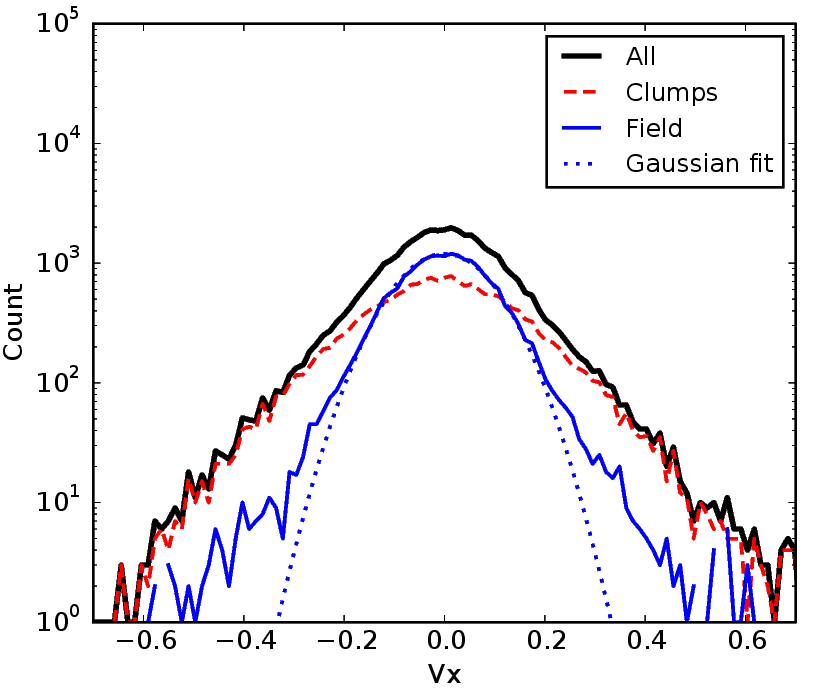
\includegraphics[width=\textwidth]{Figures/2_Vx_histogram_1}
        \caption{Distribution clumps/field}
        \label{Fig:2_Vx_histogram_1}
    \end{subfigure}
    \begin{subfigure}[b]{0.49\textwidth}
    	\centering
    	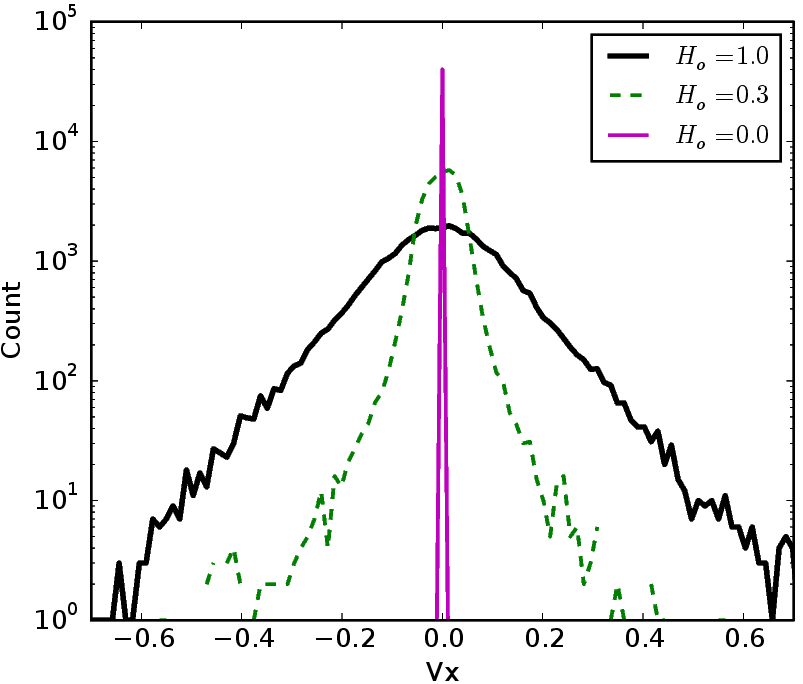
\includegraphics[width=\textwidth]{Figures/2_Vx_histogram_2}
        \caption{Distribution for different \tHub}
        \label{Fig:2_Vx_histogram_2}
    \end{subfigure}
\caption{(a) Distribution of the one-dimensional velocity field for the whole cluster as the thick solid black line, in the simulation labelled as R40h20 at the apex time (H$ = 0$). The red dashed distribution matches clump members and thin solid blue the field particles. (b) The distribution for three different values of \tHub: when $\Hub_0 = 0$, the distribution is a Dirac-$\delta$ around $v = 0$. The central distribution broadens as \tHub increases to 0.3 and 1. Observe the exponential profiles at large $|v|$. Velocities are in H.u} 
\label{Fig:2_Vx_histogram}
\end{figure}




 There is no hydrodynamics in the approach that we have taken, nevertheless expansion under gravity alone is equivalent to the adiabatic expansion of gas~: for that case, the first law of thermodynamics equates the drop in internal energy ${\rm d}U$ to minus the external work,  $-p {\rm d}V$. At constant mass, the change in gravitational energy ${\rm d}W$ is $ - {\rm d}E_k$, where $E_k$ is the kinetic energy. With $W < 0 $ but increasing over time, this implies that $E_k$ drops in amplitude. In the case when the motion is strictly radial, $E_k = 0$ when $H = 0$ and all stars come to rest. We ask to what extent the growth of substructures and non-radial motion  off-set the `adiabatic cooling' brought on by expansion. 

Fig.~\ref{Fig:2_Vx_histogram_1} graphs the x-axis one-dimensional velocity distribution for a 40k-particle model. The left-hand panel displays the overall distribution as well as the two sub-populations of clumps members and out-of-clump \textit{field} stars. We identified some 20944 stars in clumps (or $\approx $ 52\%) at the end of expansion. The expectation that all stars have zero- or low-velocities is validated by the peak in the distribution around $v_x = 0$.

As sub-structures form and  interact mutually, generating tangential as well as radial motion, the peak broadens but remains symmetric about the origin.  The large velocities are brought by stars in clumps, which demonstrates that interactions within the substructures boost the internal velocity dispersion of the cluster as a whole. Field stars dominate the low-amplitude regime. Their velocity distribution is well-fitted with a  Gaussian (shown as a dotted blue line), down to one-tenth the height of the central peak, or about 1\% of all field stars. 

To illustrate further the idea that large velocities are confined to clumps formed by fragmentation modes, we compare on Fig.~\ref{Fig:2_Vx_histogram_2} a set of models 
with different initial  values of  $\Hub_o$: 0, 0.3, and 1. 
Clearly when $\Hub_o=0$, the velocities are identically zero and there is no fragmentation whatsoever (apart from root-N noise). The distribution is then a sharp peak centered on zero. For positive but low values of $\Hub_o$, the fragmentation modes do not develop much before the apex and the (non-radial) velocities remain small. The central peak  has a much narrower dispersion, and the high-velocity wings are clipped. In this case, too, analysis of the  weakly fragmented system shows that virtually all high-velocity stars are found in clumps. The velocity distribution for the case  $\Hub_o = 1$ is added for comparison. The fact that the full range in velocities is reduced by a factor $\sim 3$ for the 
less fragmented model is also an indication of the shallower potential well of the clumps

The full population velocity distribution (solid black line) at first sight is very similar to those of \citet[Fig.~5]{Klessen2000}. In that figure, the authors show the velocity distribution of gas particles in a fragmenting system. \citeauthor{Klessen2000} attribute the high-velocity tails to gas particles falling towards stellar clumps at supersonic speed. Supersonic motions imply that gas particles trace ballistic trajectories, and hence behave like point mass particles. 

A small fraction of field stars in our calculations also have large velocities. We suspected that these stars might have acquired their large velocity through in-fall toward a nearby stellar clump. We did not, however,  find compelling evidence that would allow us to identify the origin of high velocities in field stars. Inspection of a sequence of snapshots failed to show that the velocity vectors were pointing at nearby stellar clumps: it is therefore not possible to make the same assertion as \citeauthor{Klessen2000} and state that stellar clumps accrete some field stars.

It is possible, on the other hand,  that high velocities originate from past star-star interactions. However, we did not find clear trends in the few orbits that we studied which would confirm such an event. The question of mass accretion by stellar clumps might be best settled if we added gas to our simulations to boost the mass resolution, and analysed model data using mock CCD frames, as did \citeauthor{Klessen2000}. This was not attempted here.

We close this section with a remark about the velocity distributions seen on Fig.~\ref{Fig:2_Vx_histogram} and the internal state of the stellar clumps. Because small clumps would have time to evolve dynamically through star-star collisions and reach a state of near-equilibrium (see \S\ref{Sec:Timescales}) we would expect clumps to develop a velocity field similar to Mitchie-King models of  relaxed self-gravitating star clusters \citep{BT}.  The one-dimensional velocity distribution of Mitchie-King models plotted in a logarithmic scale approaches a flat-top when $|v_{1d}|$ is small,  and cuts-off rapidly at large values~: the distributions are  concave at all velocities. This holds true for all models independently of their King parameter\footnote{Notice how this holds only because of the choice of a logarithmic vertical axis.} $W_0$. 

The shape of the distributions displayed on Fig.~\ref{Fig:2_Vx_histogram}, on the other hand, is convex as we shift, from small, to large $|v_{1d}|$. We deduce from this straightforward observation that the clumps that formed through fragmentation and subsequent mergers cannot be treated as fully in isolation and in dynamical equilibrium \`a la Mitchie-King.  Fragmentation in hydrodynamical calculations often proceeds from filaments and knots  (e.g., \citealt{Klessen2001,MacLow2004,Maschberger2010,Bate2014}). The clumps that form in a fragmenting  Hubble  flow are also surrounded by filaments and other structures which perturb them.




\subsection{The stellar mass function in clumps} 



We show on Fig.~\ref{Fig:2_ClumpMembers} the mass function of stars both in clumps, field and in the whole cluster. For brevity, we only show a model with a mass function truncated at $20 M_\odot$, however our conclusions are not sensitive to the truncation value. The mass function of $\approx 6400$ stars that were found in clumps (some 43\%) is displayed as the red solid curve and all other stars, field stars, as the blue solid curve. The theoretical Salpeter distribution function for the same number of stars is shown in black dots, with grey shades giving the  $1 \sigma$ dispersion from multiple samplings. Finally, the green dashed curve  shows the mass distribution of all 15 000 stars in the model. The lower panel is the same data normalised to the Salpeter data. 

The uptake  in massive stars for the whole population (green dashed line) of both clumps members and field stars is a statistical artefact and lie within the standard deviation of a Salpeter distribution with comparable sampling number. 

The clump member population clearly deviates from a Salpeter distribution in two ways~: first we note a deficit of low mass stars with respect to the theoretical Salpeter; secondly, although a Salpeter mass function is more or less consistent with the population up to $M\approx 2M_\odot$(black dotted line) the distribution shows a clear excess of massive stars. We find that practically all the stars more massive than 10$M_\odot$ ended up in a clump (this is the point where the solid red curve joins the dash green one). 

A linear regression fit of the clump members mass function gives a power-law index of $-2.15 \pm 0.02$, shallower than the Salpeter index of -2.35. Applying the same analysis to field stars,  we find a steeper mass function of index $-2.46 \pm 0.02$. The difference of $\approx 0.3 $ between the two populations is very similar to what is found in the Milky Way disc (see e.g. \citealt{Czekaj2014,Rybizki2015,Bastian2010} )

\begin{figure}
\begin{center}
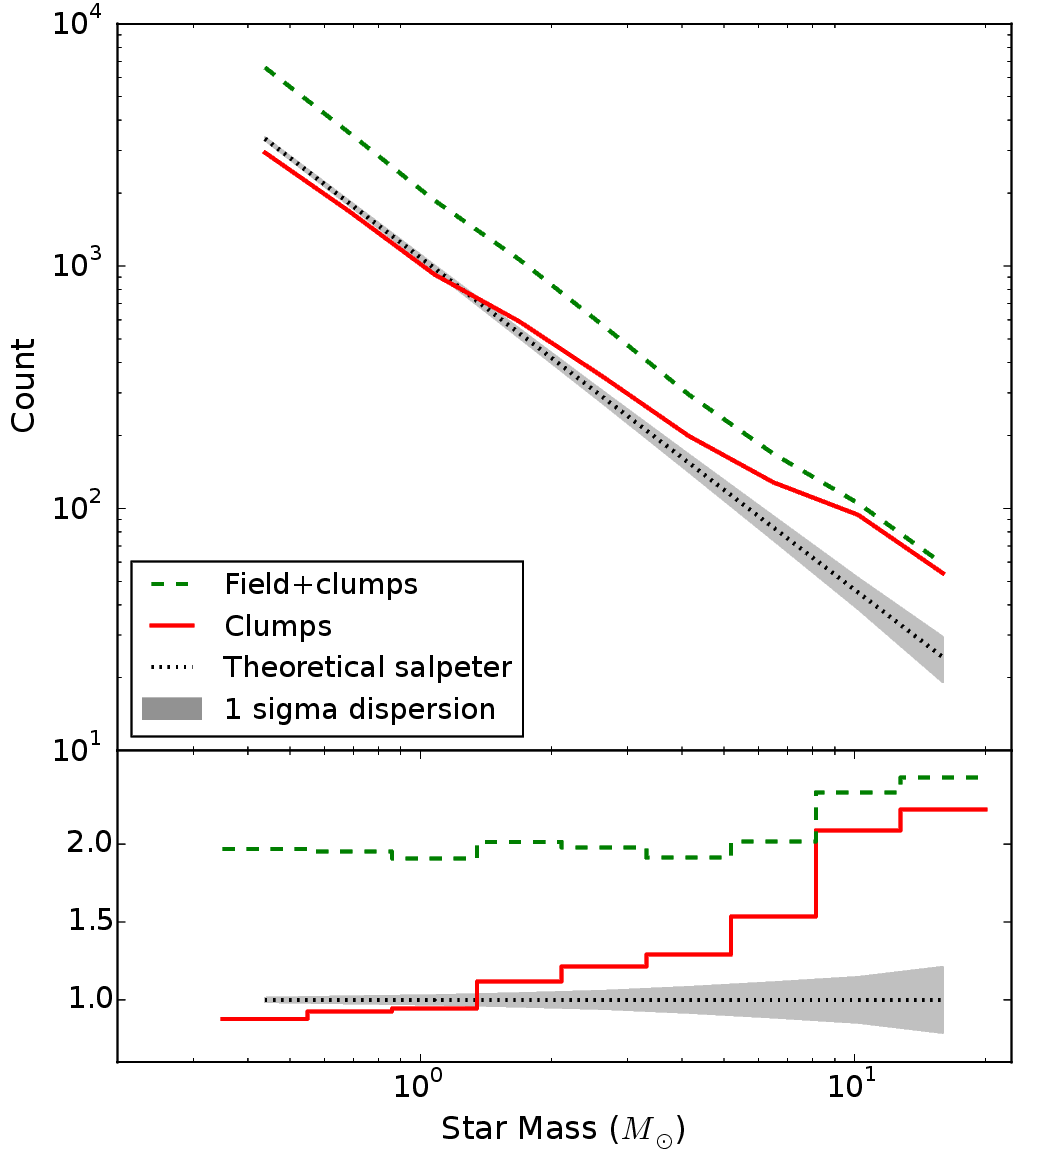
\includegraphics[width=0.8\textwidth]{Figures/2_ClumpMembers}
\caption{Top panel~: Mass function of all stars belonging to a detected clump (solid red). The expectation drawn from a Salpeter distribution function for the same total number of stars in dotted black~; the grey shade are $1\sigma$ uncertainties. The green dashed line is the  distribution for the full cluster. Bottom panel~:  same data normalised to the Salpeter expectation.}
\label{Fig:2_ClumpMembers}
\end{center}
\end{figure}

\cite{Bonnell2004} and \cite{Maschberger2010} showed from inspection of  hydrodynamical simulations that massive stars play a key role in the assembling process of clumps, attracting already formed protostars to them. We find  a similar general trend in Hubble-fragmented gas-free simulations: clumps develop around massive stars so that their stellar mass function is top-heavy. 

This excess can also be seen in the top panel of Fig.~\ref{Fig:2_MaxMass} in which for each of 440 clumps, we show as white dots the mass of their heaviest star as a function of the host clump's mass. These data were obtained from the R40h100 run. For comparison, we sampled a Salpeter mass function, drawing the same number of stars as found in each clump. We then identify the most massive star in the Salpeter sample~; the procedure was repeated 15000 times {\it for each clump} to obtain suitable statistics. The grey shades (color levels in the electronic version)  shows the resulting distribution.



 \begin{figure}
\center
    \centering
    \begin{subfigure}[b]{\textwidth}
    	\centering
    	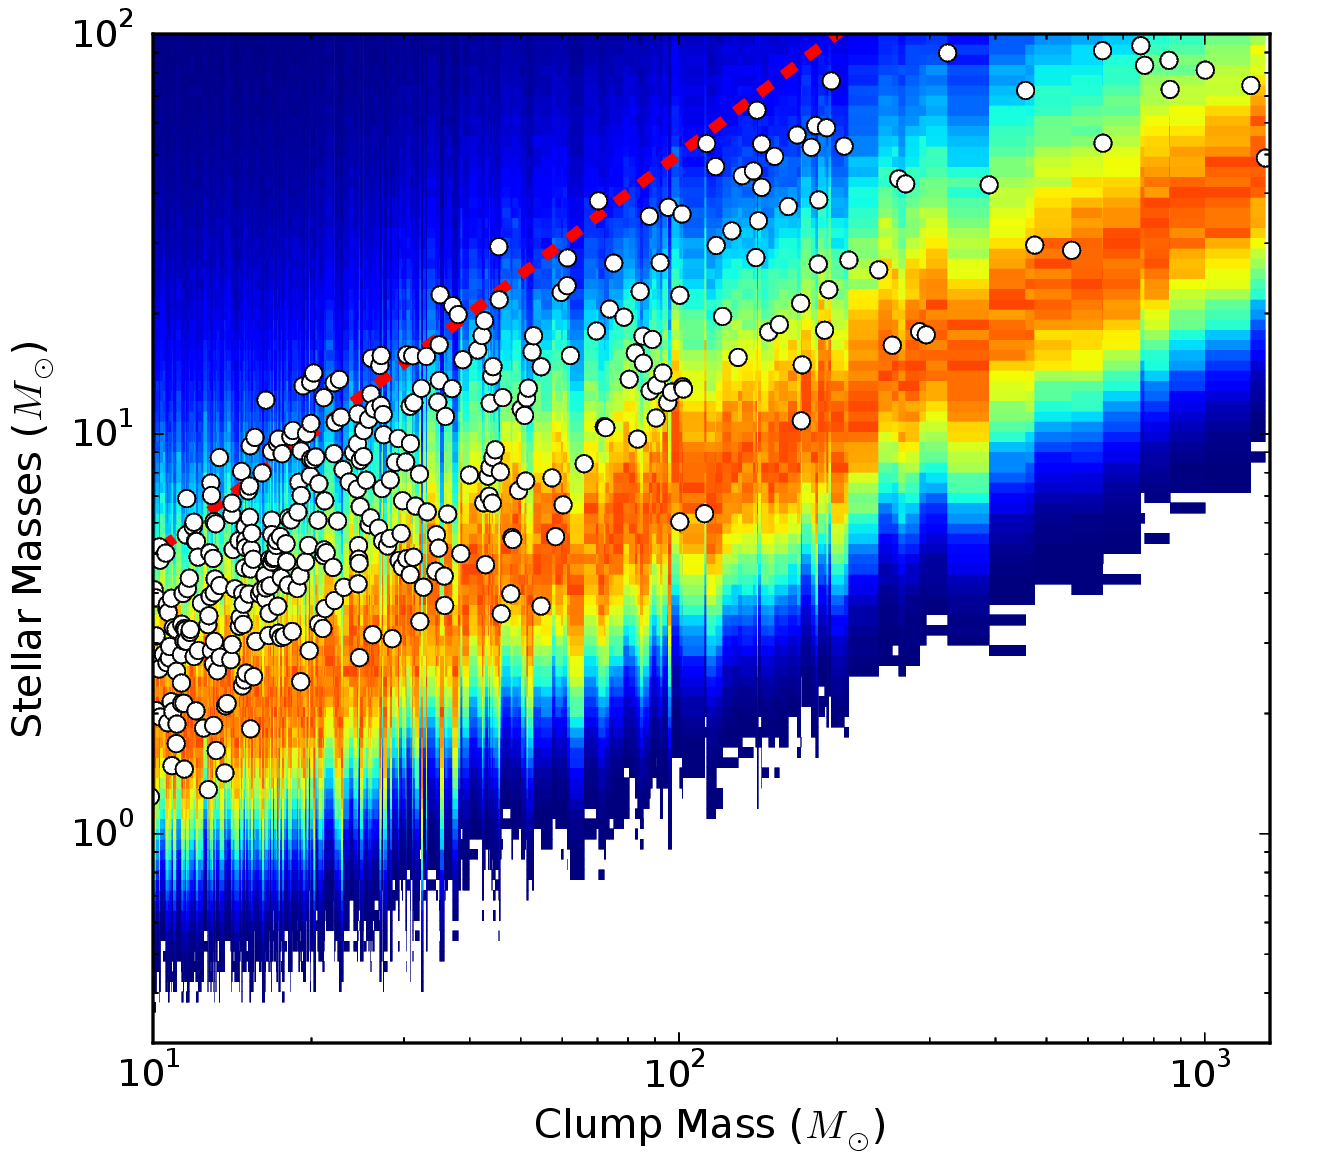
\includegraphics[width=0.7\textwidth]{Figures/2_MaxMass}
        \caption{Distribution clumps/field}
        \label{Fig:2_MaxMass}
    \end{subfigure}
    \begin{subfigure}[b]{\textwidth}
    	\centering
    	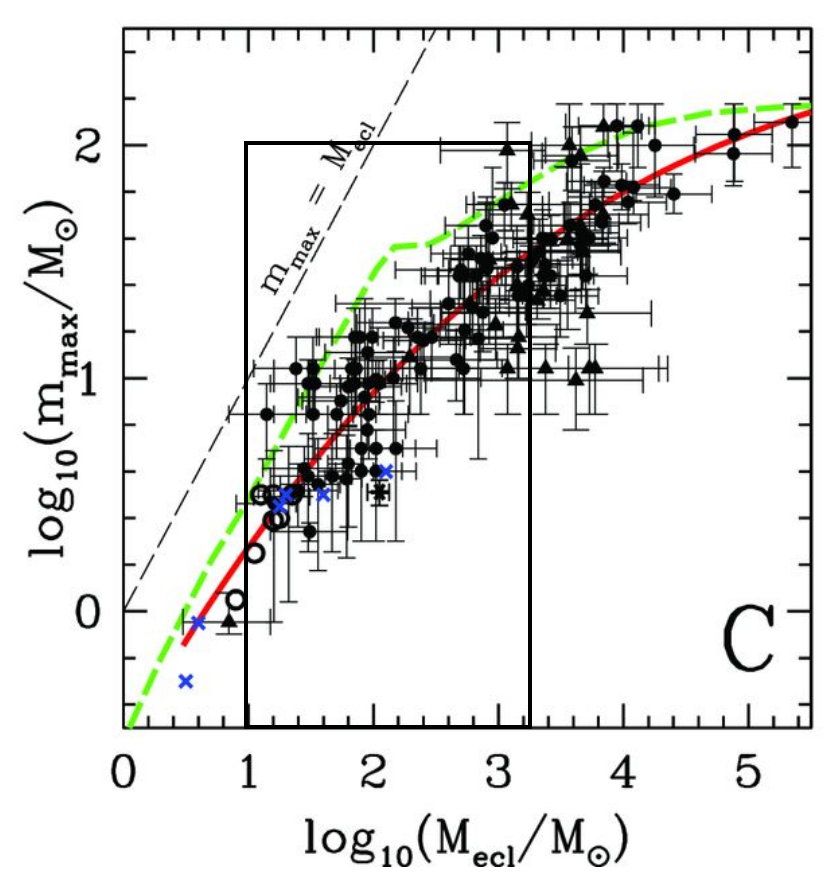
\includegraphics[width=0.6\textwidth]{Figures/2_weidner}
        \caption{Distribution for different \tHub}
        \label{Fig:2_weidner}
    \end{subfigure}
\caption{(a) Mass of the heavier star in each clump, shown as white dots, as a function of clump mass. The color map shows the likelihood for the maximum mass if all clump members were  sampled from a Salpeter IMF~; the orange crest gives the maximum likelihood. The red dashed line shows the  relation $m_{clump} = 2 m_{max}$ (see. section \ref{Sub:2_ClumpMF_MF}). The data was taken from the R40h100 run. (b) is a similar distribution from \protect\cite{Weidner2013}, built with data about young embedded star clusters from \cite{Weidner2010}. The black frame notes the range of masses displayed in (a). } 
\label{Fig:2_McMmax}
\end{figure}


 In a nutshell, Fig.~\ref{Fig:2_MaxMass} shows for each clump the likelihood that their most massive stars may be drawn from a Salpeter function, one could call the red maximum likelihood zone the "Salpeter valley". Only clumps with a mass $> 10 M_\odot$ are included to account for a possible bias when clump membership reaches below $N_d =12 $ stars. It can be seen on the figure that the scatter of white dots tends to lie systematically above the Salpeter valley. If we add the  relation $m_{clump} = 2\max\{m_\star\}$ (cf. section \ref{Sub:2_ClumpMF_MF}), we find some overlap with the data (see the red dashed line on Fig.~\ref{Fig:2_MaxMass}). This clearly illustrates the tendency for massive stars to act as seeds when the clump form, while the scatter is driven by the merger and accretion history of individual clumps. 
 
 The correlation displayed on Fig.~\ref{Fig:2_MaxMass} is in good agreement with observational data for young embedded clusters of the same mass range published by \citealt{Weidner2013}. We reproduced their figure on Fig.~\ref{Fig:2_weidner} with a black frame representing the range shown on Fig.~\ref{Fig:2_MaxMass}. 
 
 Note how the {\it scatter} in the correlation brought on by the dynamical processes at play during the adiabatic fragmentation phase also compares well with the data. Thus the stellar clumps modelled here recover an important characteristic of observed embedded young clusters.
 





\subsection{Mass segregation}
\label{Sec:2_ClumpSegregation}

In this section, we ask whether the clump assembling process at play in our simulations accounts for the mass segregation measured  in  star-forming cores in hydrodynamical simulations. The measure of mass segregation of \cite{Olczak2011} based on the MST, while efficient, will give noisy results for very small-N clumps. Instead, we follow \cite{Maschberger2010} and rank clump members according to their distance to the geometric centre of a clump, which is calculated by number-averaging (so this centre is not the clump barycentre). We then sort the bodies by mass and tabulate the radial rank of the three most massive ones. This process is illustrated on Fig~\ref{Fig:2_radial_ranking}.


\begin{figure}
\begin{center}
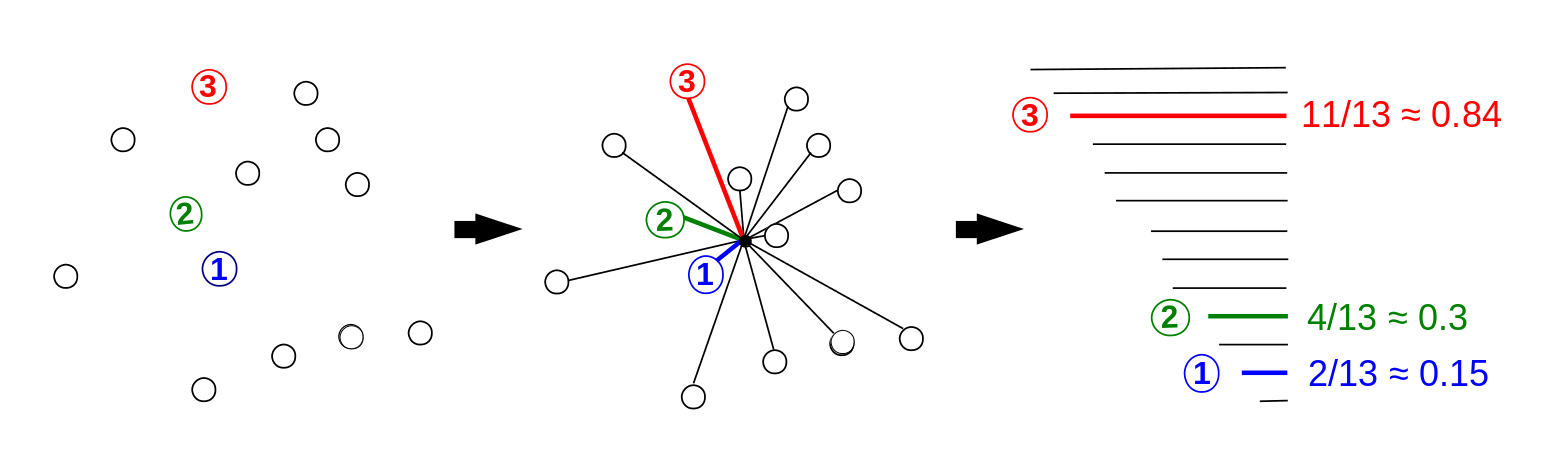
\includegraphics[width=\textwidth]{Figures/2_radial_ranking_schema}
\caption{Illustration of the radial ranking method. Stars marked 1,2 and 3 are the first, second and third most massive stars in the clump. Distances to the geometrical center are computed then sorted. The position in the sorted list is converted to a number, the radial rank.}
\label{Fig:2_radial_ranking}
\end{center}
\end{figure}

The great advantage of this approach is that it is independent of geometry and absolute size once the ranking is normalised to the clump membership $N_c$.  One issue arises with the binning of the rank, since small values of $N_c$ give large intervals by construction, and conversely for populous clumps~: we found a good compromise by setting the width of each bin to 1/20 since the mean clump mass $\sim 20 M_\odot$ implies $N_c \sim 20$ on average. The procedure is repeated over all clumps identified in the run (typically on the order of $\sim 200$). The diagnostic for an un-biased sampling is a profile with radius that remains the same regardless of the mass selected~; if, furthermore, the stars are (on the mean) un-segregated in radius, then the profiles will be flat. 


Fig.~\ref{Fig:2_ClumpSeg} graphs the  distribution of rank of the three most massive stars in all the clumps from R40h100 fragmented state. The salient features are that 1) none of the distributions are flat, all three peaking significantly  at small ranks~; and 2) there is a clear trend for the most massive star also to be the most  segregated. Precisely this result had to be expected from the internal dynamics of small clumps (cf. section~\ref{Sec:Timescales}).  Our Fig.~\ref{Fig:2_ClumpSeg} should be compared with Fig.~13 of \cite{Maschberger2010}: the authors also found radial rank distribution to peak at small values for massive stars, showing a level of mass-segregation in their clumps.

It is striking that the measure of mass segregation attained here for a gas-free configuration is a good match to a full hydrodynamical setup. By implication the segregation proceeds more vigorously once the proto-stellar cores have condensed and behave essentially like point sources. The initial configuration that we have adopted relies only on density fluctuations to seed clumps, however once again we find evidence that massive stars begin and remain the centre of gravitational focus for clump formation. That is not so when clumps are setup using a fractal approach \citep{Goodwin2004,Allison2009}. There is then no segregation initially, and it all develops at or shortly prior to the global system evolution towards equilibrium (the collapsing violent relaxation phase). 


\begin{figure}
\begin{center}
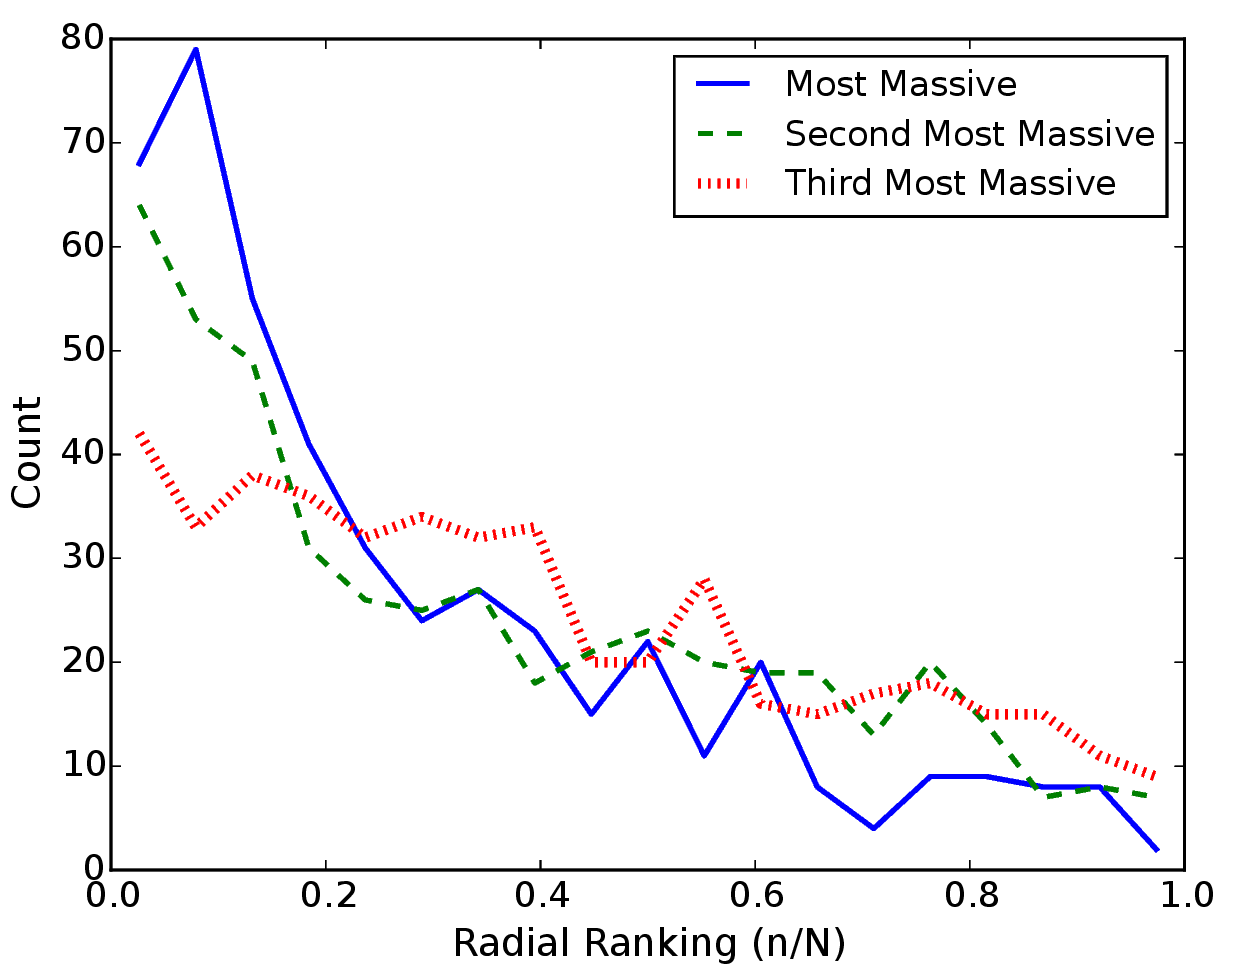
\includegraphics[width=0.6\textwidth]{Figures/2_ClumpSeg}
\caption{Histograms of radial ranking of first, second and third most massive star in each clump for a model with N = 40 000 stars (R40h100).}
\label{Fig:2_ClumpSeg}
\end{center}
\end{figure}







\section{Concluding remarks}
In the next section we follow through with the final stage of evolution towards equilibrium and compare the final configuration with those of \cite{Allison2009} and the recent study by \cite{Caputo2014}. 